% Two-page submission, drafted by Claude for Salah's revision (2026-11-21), in the
% voice of Salah's English notes (first person, plain section titles, quotes of the
% sources in footnotes, a closing "Clarifications" section).
% Passages in violet (\interp{...}) are interpretations or statements about the author:
% Salah confirms, rewrites or removes each of them. [AV] marks a claim about another
% paper to check at the source. The extended version is report_extended.tex.
% Compile with: tectonic report.tex
\documentclass[10pt]{article}
\usepackage[utf8]{inputenc}
\usepackage[T1]{fontenc}
\usepackage[english]{babel}
\usepackage[a4paper, margin=1.7cm, top=1.2cm, bottom=1.3cm]{geometry}
\usepackage{amsmath}
\usepackage{graphicx}
\usepackage{booktabs}
\usepackage{xcolor}
\usepackage[font=footnotesize, labelfont=bf, skip=3pt]{caption}
\usepackage{hyperref}
\hypersetup{colorlinks=true, urlcolor=blue, linkcolor=blue, breaklinks=true}
\graphicspath{{../figures/}}
\tolerance=2000
\setlength{\emergencystretch}{3em}
\setlength{\parskip}{1pt}
\setlength{\textfloatsep}{6pt}
\setlength{\floatsep}{4pt}
\setlength{\footnotesep}{6pt}
\makeatletter
\renewcommand\section{\@startsection{section}{1}{\z@}{-1.2ex}{0.5ex}{\normalfont\normalsize\bfseries}}
\renewcommand\@makefntext[1]{\noindent\footnotesize\textbf{\@thefnmark.}\ #1}
\makeatother
\renewcommand{\thesection}{\arabic{section}.}
\newcommand{\interp}[1]{\textcolor{violet}{#1}}
\newcommand{\av}{\textcolor{red}{[AV]}}

\begin{document}

\begin{center}
{\small Mechanistic Interpretability Hackathon 5: Autointerp}\\[2pt]
{\large\bfseries Do autointerp scorers agree? Five LLM scorers, one SAE, and a placebo}\\[2pt]
{\small \textbf{Salah Chadli} $\cdot$ 21 November 2026 $\cdot$
\url{https://github.com/chadlis/scorer-agreement}}
\end{center}

\section{The starting point}

In automated interpretability (\emph{autointerp}), a sparse autoencoder (SAE) splits
the activations of a language model into many \emph{features}, and an LLM writes a short \emph{explanation} of each feature. To evaluate
an explanation, the \emph{detection} method of Paulo et al.\ (2024) shows it to a
second LLM, the \emph{scorer}, together with a short text: the scorer answers 1 if it
predicts that the feature fires on the text, and 0 otherwise. The share of right
answers is the score of the explanation.

This score therefore depends on two things: the explanation, which one wants to
measure, and the scorer, which is a choice of the pipeline. Van der Ben et al.\ (2026)
show that the choices of the pipeline make autointerp scores vary a great deal, and
they keep a single scorer fixed, Gemini Flash\footnote{``All scoring uses Gemini Flash
as the fixed scorer, isolating explainer identity from scorer variation.'' Van der Ben
et al.\ 2026, section 2. \av}. Chen (2026), for his part, shows that a rule that never
reads the explanation can do better than LLM scorers on stored scoring data, and he
recommends reporting every score beside such a rule\footnote{``Scores should be
reported beside the best explanation-free rule on the same items.'' Chen 2026,
abstract. \av}. Scorers have already been compared: Paulo et al.\ (2024, section 4.1
and appendix F.7) score the same explanations with three scorers, but compare them
through their mean scores and the correlations of their scores \av.

\section{The question}

I formulate the question as follows: \emph{with texts and explanations held fixed, do
scorers differ in their judgments, and in the gain that the explanation brings them
over the explanation of an unrelated feature (a placebo)?} To my knowledge (searches
of 17 and 21 November 2026), no study measures, for several detection scorers, their
agreement text by text, the gain that each of them draws over an explanation-free
control, and whether their disagreements change which explanation is preferred.

This work makes three contributions. First, it measures how often five scorers disagree
on the same text (7 to 13\% of the texts for a pair), and not only whether their mean
scores agree. Second, it compares the gains of the scorers over the placebo pair by pair,
on the same texts (four gain about the same, Opus about 3 points more). Third, in an
exploratory analysis decided after the results, it asks whether the disagreements change
which of two explanations a researcher would keep (opposite choices on 13 to 27\% of the
features for a pair).

\section{What I did}

The design was frozen in git before the first scorer call (tag \texttt{plan-frozen}).
I drew 100 features of the SAE \texttt{gpt2-small/6-res-jb} (Neuronpedia), with a
published seed, among those that fire on 0.001\% to 1\% of tokens and have two original
explanations (A by gpt-3.5-turbo, B by gpt-4o-mini). Each feature has 40 texts of 17
tokens, 20 \emph{positives} and 20 \emph{negatives}. Every label is measured, by
recomputing the activation of the feature on the exact text shown: a positive reaches
at least 10\% of the maximum of the feature, from the weakest to the strongest, and a
negative is exactly 0. The negatives are stored windows of the other sampled features,
so that positives and negatives share the corpus, the length and the cut, and no token
is marked. Each text is scored under A, under B and under the placebo. The scorers are
Claude Haiku 5.5, Sonnet 5.5 and Opus 5.5, Gemini 2.5 Flash and Mistral Small 3.2, with
the detection prompt of delphi and the most deterministic settings each model accepts.
The \emph{gain} is the accuracy with A and B minus the accuracy with the placebo.
Intervals are 95\% bootstrap intervals over features.

\section{What I found}

\begin{figure}[h]
\centering
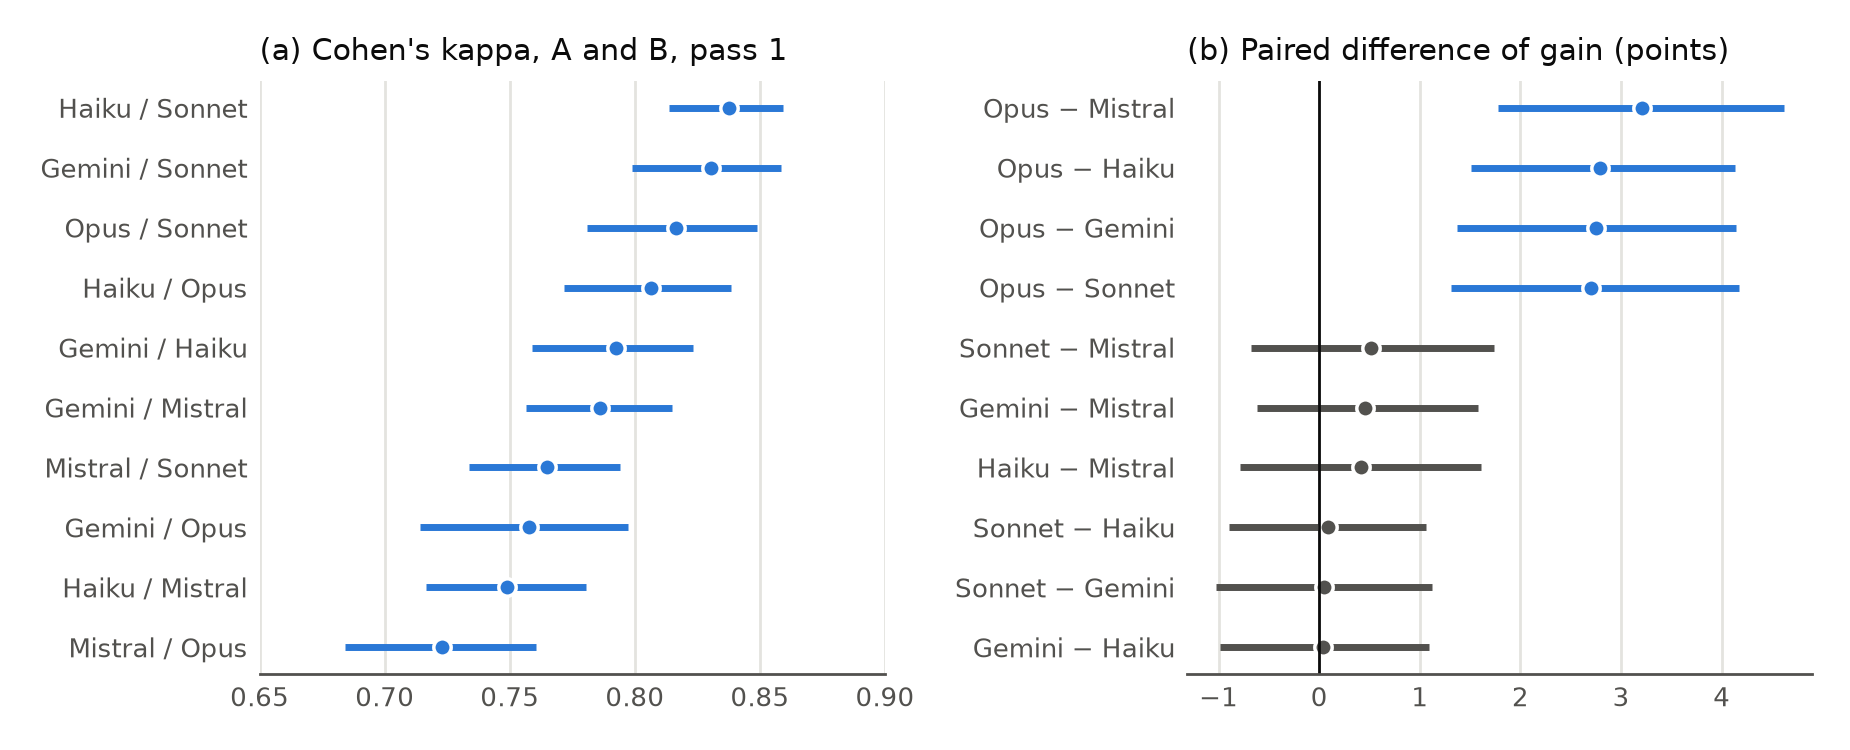
\includegraphics[width=0.84\linewidth]{fig_report_main.png}
\caption{The two central measures, with 95\% bootstrap intervals over features. (a)
Cohen's kappa of each pair of scorers, explanations A and B, pass 1, about 7,900 texts
per pair. (b) The 10 paired differences of gain over the placebo, each oriented as
larger minus smaller, in blue when the interval excludes 0. The gains are in
Table~\ref{tab:profile}.}
\label{fig:main}
\end{figure}

\textbf{Judgments.} The raw agreement goes from 86.9\% (Mistral and Opus) to 92.6\%
(Haiku and Sonnet), and Cohen's kappa from 0.72 to 0.84, with intervals that do not
overlap for the extreme pairs (Figure~\ref{fig:main}a). Each scorer changes its own
answer between two passes on only 0.1 to 3.1\% of the texts: these disagreements are
therefore not sampling noise.

\textbf{Gain.} The placebo works as a control: every scorer falls to chance (48.6 to
49.5\%), so the texts carry no usable cue of their label.
With the explanations, the accuracy rises to 77 to 83\%, a gain of about 30 points for
every scorer (29.2 to 32.4, Table~\ref{tab:profile}). Six of the ten paired differences
lie between $-0.1$ and $+0.5$ points, with intervals of about $\pm1.2$ points: Haiku,
Sonnet, Gemini and Mistral draw a similar benefit from the explanation, although no
margin of equivalence was set in advance (Figure~\ref{fig:main}b). The four other
differences are those of Opus, which gains about 3 points more than each of the others
(Opus minus Mistral: $+3.2$, [1.8, 4.6]). They still exclude 0 with Bonferroni
intervals that hold together at 95\% (Opus minus Mistral: [1.2, 5.2]).

\begin{table}[h]
\centering
\footnotesize
\begin{tabular}{lrrrrrrrrr}
\toprule
& Gain & \multicolumn{3}{c}{Sensitivity (\%)} & \multicolumn{3}{c}{Specificity (\%)} & Invalid & Changed \\
\cmidrule(lr){3-5}\cmidrule(lr){6-8}
Scorer & (pts) & A & B & placebo & A & B & placebo & (\%) & (\%) \\
\midrule
Haiku 5.5 & 29.6 & 62.1 & 67.1 & 1.5 & 92.2 & 91.5 & 95.9 & 1.2 & 3.1 \\
Sonnet 5.5 & 29.7 & 60.3 & 67.4 & 1.1 & 94.9 & 94.2 & 98.0 & 0.2 & 1.4 \\
Opus 5.5 & 32.4 & 71.2 & 75.0 & 2.1 & 90.1 & 90.0 & 96.2 & 0.9 & 2.3 \\
Gemini 2.5 Flash & 29.6 & 58.7 & 65.6 & 1.2 & 95.7 & 96.2 & 97.6 & 0.2 & 0.2 \\
Mistral Small 3.2 & 29.2 & 60.9 & 63.6 & 1.2 & 93.6 & 94.6 & 96.8 & 0.6 & 0.1 \\
\bottomrule
\end{tabular}
\caption{Profile per scorer, mean of both passes. Sensitivity: positives answered 1.
Specificity: negatives answered 0. Invalid: unreadable after one retry. Changed: texts
answered differently by the two passes.}
\label{tab:profile}
\end{table}

\textbf{Where the differences come from.} With as many positives as negatives, the
gain splits into two parts,
$\tfrac12(\text{sens}_{AB}-\text{sens}_P)+\tfrac12(\text{spec}_{AB}-\text{spec}_P)$.
For every scorer, the first part makes the gain (30.5 to 35.5 points) and the second
is a small loss (0.8 to 3.1 points). In other words, the explanation makes a scorer
find many more positives, and raise a few more false alarms (Table~\ref{tab:profile}).
Opus finds 73\% of the positives, against 62 to 65\% for the others, and answers 1 to
about 10\% of the negatives, against 4 to 7\%. \interp{Its larger gain therefore seems
to me to come from a lower threshold for answering ``yes'', rather than from a better
reading of the explanation.}

\textbf{The texts where the scorers disagree.} The five scorers are not unanimous on
1,568 texts (20\%). I drew 30 of them, and two fresh LLM agents, blind to the names of
the scorers but not to the labels, proposed a cause for each disagreement. They agree on 25 of the 30 (kappa 0.79), and
they attribute 18 to 21 of them to the explanation or the text rather than to an error
of the scorer. For example, a feature explained as ``references to radio'' fires on
``Radio'' in ``Radioactive Man'', and the lone scorer that answers 1 is right. These
causes are hypotheses rather than measurements. My own reading broadly agrees, but I
did not record it text by text.

\textbf{Do the scorers pick the same explanation?} This analysis is exploratory and was
decided after the results (DEVIATIONS.md, entry 2). Across the 200 explanations, the
scorers rank the accuracies alike (Spearman 0.76 to 0.90). Choosing between A and B
for a given feature is less stable: two scorers pick opposite explanations on 13\%
(Haiku and Sonnet, [7, 20]) to 27\% (Opus and Gemini, [18, 36]) of the features, while
a scorer compared with itself, pass 1 against pass 2, does so on 0 to 7\%. On 47 of the
100 features, at least two scorers prefer opposite explanations. These preferences
rest on 40 texts per feature.

\section{What this allows me to say}

\interp{I can thus conclude that, on this SAE and with this prompt, the five scorers
draw a similar average benefit from an explanation, within about 3 points, while two
of them disagree on about one text in ten. The larger gain of Opus
comes with more false alarms, and much of the disagreement seems to come from
explanations that do not describe the feature exactly. Finally, the scorers rank the
explanations alike overall, but on almost half of the features at least two of them
would keep a different one of the two explanations.} It will then remain to score new
texts for the same explanations, comparing one scorer on two disjoint sets of texts
with two scorers on the same set, in order to tell whether these reversals come from
the scorer or from the choice of the texts.

\section{What this does not show}

High agreement is not validity: scorers can be wrong together. A gain shows that the
explanation helps to predict activations, not that it describes a mechanism. The study
covers one SAE, one layer, 100 features and one prompt, with three Claude models among
the five scorers, and with settings that differ by scorer, so that a difference mixes
the model and its setting. The positives come from stored examples, and nothing reliable
can be said about A against B for a given feature.

\section*{Clarifications}

\textbf{Prior work.} The setup, the prompt, the draw, the placebos and the code were
prepared before the kick-off (20 November, 18:00), and every scorer call and analysis
was made on 21 November (27.55 USD). \textbf{Reading status.} \interp{At this stage,
I have read [to complete: which of the three papers I have read in full, and which only
through summaries].} \textbf{Use of AI.} \interp{The code, the figures, the layout and a
first draft of this text were produced with Claude Code (Claude Opus 5.5), from my
design decisions and my reading of the results. I revised the text.}

{\footnotesize\noindent\textbf{References.} Chen, X. (2026). \emph{Scoring explanations
without reading them: structural shortcuts in automated-interpretability evaluation
data}. arXiv:2610.37676. Paulo, G., Mallen, A., Juang, C. and Belrose, N. (2024).
\emph{Automatically interpreting millions of features in large language models}.
arXiv:2410.13928. Van der Ben, S., Roch, N., Hedstr\"om, A. and El-Assady, M. (2026).
\emph{Building fast, evaluating slow: pipeline choices dominate autointerpretability
score variance}. arXiv:2607.19386.\par}

\end{document}
